\documentclass[10pt,a4paper]{article}
\usepackage[margin=22mm]{geometry}
\usepackage{fontspec}
\usepackage{newunicodechar}
\newunicodechar{τ}{\ensuremath{\tau}}
\usepackage{booktabs,array,graphicx,titlesec,enumitem}
\usepackage[hyphens]{url}
\usepackage[hidelinks]{hyperref}
\setlength{\parskip}{3pt}
\setlength{\emergencystretch}{2em}
\clubpenalty=10000
\widowpenalty=10000
\urlstyle{same}
\titleformat{\section}{\large\bfseries}{}{0pt}{}
\titleformat{\subsection}{\normalsize\bfseries}{}{0pt}{}

\hypersetup{pdftitle={Resource-Efficient Local Language Models for Agricultural Tasks: A 9B–27B Comparison with Deterministic Tools},pdfauthor={Antoniy Sarychev; Denis Shesternin}}
\begin{document}
\begin{center}\bfseries\large Resource-Efficient Local Language Models for Agricultural Tasks: A 9B–27B Comparison with Deterministic Tools\end{center}
\begin{center}Antoniy Sarychev, Denis Shesternin\end{center}
\begin{center}Russian State Agrarian University — Moscow Timiryazev Agricultural Academy, Moscow, Russia\end{center}
\begin{center}\emph{Working draft, 5 October 2026. Final approval by both authors and the manuscript license are pending. The Russian and English texts are versions of one study.}\end{center}
\section*{Abstract}
We examine the quality, latency and memory tradeoff of two practical local language-model configurations on one consumer PC, and distinguish tool declaration from completed deterministic execution. On the public development split of MERA ruTXTAgroBench, Qwen3.5-9B Q8\_0 and Qwen3.8-27B UD-Q4\_K\_M attain strict option-set exact match of 141/289 and 150/289, respectively; four original references remain unresolved. A separate native-interface TELEMETRY40 run is scored retrospectively: exact match is 22/39 versus 24/39, with median request latency of 0.269 versus 1.434 seconds and sampled whole-GPU peaks of 11,471 versus 13,287 MiB. Input texts and recorded weight hashes agree with the historical run, but schema, seed, checkpoint caching and GPU placement differ, and some choices change; we therefore report full-split quality and native telemetry separately. In a live constructed calculation study, full correctness is 7/27 versus 18/27 for Qwen9 without and with tools, and 15/27 versus 25/27 for Qwen27; both tool arms reach 16/16 numeric answers, while clarification errors remain. These development observations support a bounded configuration tradeoff, without establishing equivalence, a causal parameter-count effect, or the safety of agricultural advice.

\textbf{Keywords:} local language models; agricultural benchmarks; resource efficiency; deterministic computation; tool execution; reproducibility.

\section*{1. Research problem and contribution}
Local agricultural assistants face both knowledge questions and precisely specified calculations. The first may require domain knowledge; the second can often be checked against an explicit formula and units. A small local model may reduce latency and occupied memory, yet a plausible output or a correctly named tool can still conceal an incorrect answer. Deployment decisions therefore require evidence about the complete evaluated configuration and the computation actually executed.

We ask three questions. First, what quality–resource tradeoff is observed between Qwen3.5-9B and Qwen3.8-27B on a consumer PC? Second, how does model-only calculation compare with actual execution of allowlisted deterministic tools? Third, as a supplementary question that may have a negative or inconclusive answer, what do existing cloud-escalation experiments show? The configurations differ in model generation, size, quantization and memory placement, so the design does not isolate the causal effect of parameter count.

The contribution is an auditable development case study: a preserved agricultural benchmark comparison, a retrospective compatibility check linking saved predictions to telemetry, and a separately identified calculation experiment. The hidden MERA TEST split was not used. The 9B configuration is the focal practical option and the 27B configuration a reference with higher observed quality; no acceptable quality loss was defined in advance.

\section*{2. Related literature}
FrugalGPT, AutoMix, Hybrid LLM, RouteLLM and the unified routing-and-cascading framework formalize model selection and escalation [1–5]. RouterBench separates cached-output comparisons from the behavior and cost of a deployed router [6]. These methods motivate measuring the resources of the actual serving configuration, but their published gains do not transfer automatically to our models, data or hardware; our own saved-output routing analyses remain exploratory replay.

Semantic Entropy Probes and the abstention survey show that reliability requires a defined uncertainty or refusal criterion [7, 8]. An output confidence field, a lexical support check or a grammatical JSON object cannot by itself establish correctness. We therefore report format compliance, transport completion, option-set quality and input clarification separately.

PLLaMa, AgriGPT and AgroLLM investigate agricultural adaptation and knowledge transfer [9–11]. AgriAgent and AgroTools address agricultural planning and tool orchestration [12, 13], so agriculture combined with tools is already an established direction. Our narrower comparison concerns local resources and the difference between a declared and an executed calculation. τ-bench evaluates completed interaction goals, and ToolACE studies function-calling data and validation [14, 15]; both motivate our complete-answer rather than tool-name-only scoring.

Efficient architectures and quantization also require careful identity control. BitNet describes native low-bit models, and the Gemma 4 report covers dense and mixture-of-experts architectures [16, 17]; neither supplies measurements for the third-party GGUF configurations studied here. AgXQA offers a different agricultural question-answering setting [18], used only in earlier HOME experiments. For computation we rely on the FAO-56 equations and units [19]. The MERA evaluation platform is described in [20]; the ruTXTAgroBench task page is listed separately as a technical source [T1].

\section*{3. Data, configuration and analysis}
\subsection*{Separate evidence blocks}
MERA ruTXTAgroBench contains 2,935 Russian multiple-choice questions across ten agricultural disciplines, including 293 public DEV items [20, T1]. Its creators describe agricultural-expert authorship, professional editing and checking by three experts. This is attributed methodology, not our independent verification of every key or of farm-level applicability. Questions, gold labels and unrestricted benchmark logs are kept outside the editorial package and software release, in line with the dataset restrictions.

The initial balanced DEV60 screen is contained in DEV293, so model selection and earlier prompt and scorer inspection affect the full-split results. TELEMETRY40 selects four positions per discipline from the same DEV without inspecting reference answers; twenty of its IDs also occur in DEV60, and it is not independent validation. Study C contains 27 constructed Russian development cases in repeated formula families. HOME150 is a separate earlier controlled study with bilingual and synthetic cases. The accuracies of these blocks are never combined.

\subsection*{Scoring and denominator policy}
Our strict metric parses a set of Latin option identifiers, checks membership in the supplied options, and requires exact set equality for EM. Per-item set F1 is the harmonic mean of precision and recall, and tables report its macro average. Four original DEV references mix Cyrillic and Latin identifiers and cannot be resolved under the declared parser; they remain unresolved, without inferred transliteration or changed labels. Main quality estimates use 289 scored references; all 293 attempted outputs and a conservative all-item sensitivity are retained.

The published MERA scorer is treated as a separate diagnostic. Its SQuAD-derived normalization can remove Latin A as an English article and responds differently to order and spacing. The production-server scoring implementation could not be independently verified; therefore the locally reproducible strict set metric is reported separately from official MERA scoring, and strict EM/F1 are not described as official MERA scores.

Paired outcomes and the retained discipline-stratified bootstrap are descriptive analyses of reused DEV. No numerical non-inferiority margin was specified for the 9B–27B comparison, and the interval cannot remove model-selection effects or prove equivalence.

\subsection*{Hardware and profiles}
The measured machine has an AMD Ryzen 7\,8700F, an RTX 5060 Ti reporting 16,311 MiB VRAM, and 31.620 GiB system RAM. Recorded software is Windows 11 Pro, NVIDIA driver 617.14 and LM Studio 0.4.25+1, with the globally selected llama.cpp CUDA12 runtime 2.51.0; the exact engine build per model is not exposed. The main GGUF files are 8.873 GiB for Qwen9 Q8\_0 and 15.334 GiB for Qwen27 UD-Q4\_K\_M. File identity comes from SHA-256 receipts, not from a serving catalogue's aggregate size or a hosted display name.

Historical DEV quality used OpenAI-compatible requests, a strict response schema, seed 42, context 2,048, temperature zero, top\_p one, at most 512 output tokens, and disabled reasoning. Loading requested GPU placement max for Qwen9 and 0.75 for Qwen27, with checkpoint caching 32 and periodic reloads; actual offloaded layer counts were not measured. Reasoning-disabled, short-output multiple-choice results do not represent unconstrained reasoning quality.

Native TELEMETRY40 uses LM Studio's native REST interface with the same recorded input texts, context, temperature, top\_p and token limit, but no exposed seed or server-side schema enforcement. It disables reasoning and MTP, sets checkpoint caching to zero, enables flash attention and requests automatic GPU placement. ABBA blocks, one synthetic warmup per load, serial inference and explicit unloads limit operational drift. Load and warmup time are reported separately from request latency and do not characterize cold-load distributions.

Memory is sampled in three scopes: whole-device GPU use, whole-system used RAM and named LM Studio process-group RSS. Background applications, shared pages and process selection affect these scopes, so they do not measure model-private allocation. Request latency is the client HTTP round trip; client and backend time to first token (TTFT) are distinct. Output rates on short answer-letter tasks do not establish long-form generation speed, and energy use was not measured.

\section*{4. Quality and resource results}
\par\smallskip\noindent\begin{minipage}{\linewidth}\noindent{\small Table 1. Historical DEV293 quality under the OpenAI-compatible profile. All 293 requests completed for both configurations; 289 references are parseable.\par}\nopagebreak\vspace{3pt}
{\centering\small \setlength{\tabcolsep}{4pt}
\begin{tabular}{@{}>{\raggedright\arraybackslash}p{0.33\linewidth}>{\centering\arraybackslash}p{0.24\linewidth}>{\centering\arraybackslash}p{0.12\linewidth}>{\centering\arraybackslash}p{0.25\linewidth}@{}}
\toprule
Configuration & Strict EM & Macro set F1 & Latency p50 / p95, s \\
\midrule
Qwen3.5-9B Q8\_0 & 141/289, 48.79\% & 0.6286 & 0.295 / 0.402 \\
Qwen3.8-27B UD-Q4\_K\_M & 150/289, 51.90\% & 0.6468 & 1.374 / 1.753 \\
\bottomrule
\end{tabular}\par}\end{minipage}\par\medskip
The observed Qwen9 minus Qwen27 EM difference is −3.11 percentage points. Paired outcomes are 113 correct for both, 28 only for Qwen9, 37 only for Qwen27 and 111 incorrect for both. The retained 10,000-repeat discipline-stratified bootstrap gives a descriptive 95\% interval of [−8.30, +2.42] points for the EM difference and [−0.06148, +0.02552] for the F1 difference. The ratio 141/150 = 94\% describes relative observed EM: Qwen9 accuracy is 48.79\%, and equivalence is not established. Assigning unresolved references zero yields a conservative sensitivity of 141/293 = 48.12\% and 150/293 = 51.19\%, which does not resolve their truth.

\par\smallskip\noindent\begin{minipage}{\linewidth}\noindent{\small Table 2. Native TELEMETRY40 outputs and resources from one saved run. Quality is scored retrospectively on 39 parseable references; timing and memory cover 40 completed requests per model.\par}\nopagebreak\vspace{3pt}
{\centering\small \setlength{\tabcolsep}{4pt}
\begin{tabular}{@{}>{\raggedright\arraybackslash}p{0.5\linewidth}>{\centering\arraybackslash}p{0.22\linewidth}>{\centering\arraybackslash}p{0.22\linewidth}@{}}
\toprule
Measurement & Qwen9 & Qwen27 \\
\midrule
Strict EM & 22/39, 56.41\% & 24/39, 61.54\% \\
Macro set F1 & 0.7197 & 0.7801 \\
Request p50 / p95, s & 0.269 / 0.344 & 1.434 / 1.829 \\
Client TTFT p50, s & 0.122 & 0.691 \\
Whole-GPU sampled request peak, MiB & 11,471 & 13,287 \\
Whole-system RAM sampled request peak, GiB & 20.858 & 28.470 \\
Process-group RSS sampled request peak, MiB & 11,198.96 & 18,742.34 \\
Transport completion / JSON presentation violations & 40/40 / 2 & 40/40 / 0 \\
\bottomrule
\end{tabular}\par}\end{minipage}\par\medskip
On these native requests, Qwen9 has 5.338 times lower median latency, while Qwen27 answers two more scored questions correctly. Neither configuration dominates in all displayed criteria; the result is a descriptive tradeoff, not a universal winner (Figure 1).

The retrospective audit finds exact agreement of system and user input bytes for all 80 historical/native pairs and agreement of recorded weight identities. Parsed option choices nevertheless change for 1/40 Qwen9 and 2/40 Qwen27 items, and historical quality on the same subset is 23/39 for each model (F1 0.7282 and 0.7374). Runtime and interface differences therefore constrain comparability: full DEV293 quality must not be attached to native speed as if both were measured jointly under identical settings. Native subset quality and timing can be reported together, provided their retrospective, selected-development status is explicit.

\begin{figure}[ht]\centering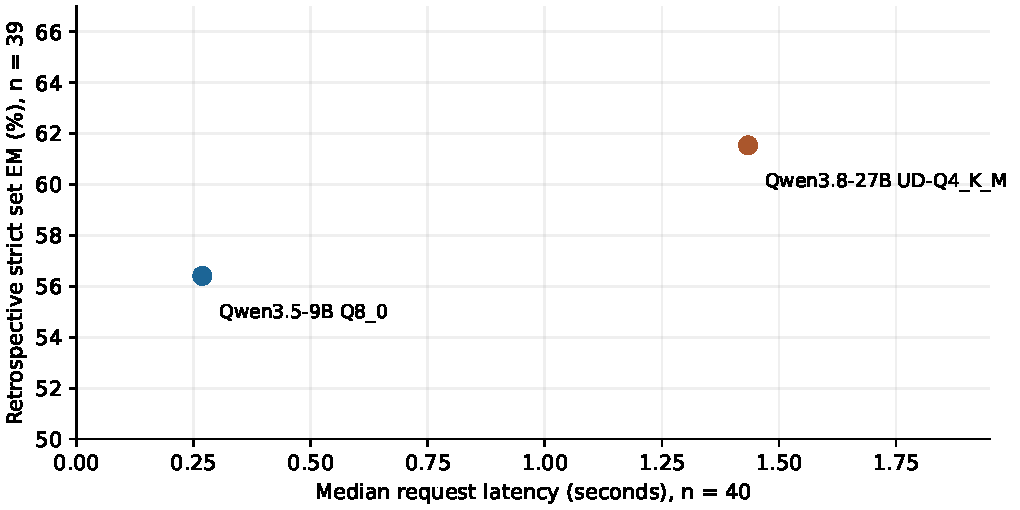
\includegraphics[width=0.9\linewidth]{../results/20261004_article_build/native40_tradeoff.pdf}\par\smallskip{\small Figure 1. Native TELEMETRY40: retrospective strict EM on 39 references versus measured request latency on 40 calls. Both configurations reuse DEV; the point values do not establish equivalence or a causal size effect.\par}\end{figure}
The initial native profile with 32 checkpoints produced RAM-guard-censored Qwen27 attempts. A subsequent checkpoint-zero profile completed TELEMETRY40, and all original failures remain archived. These were operational failures, not answer errors. The absence of further errors characterizes the observed runs, not long-term reliability or reproducibility across machines.

\section*{5. Calculations and completed tool execution}
Study C supplies a typed task name, question, public numeric inputs and explicit units to every arm. It covers simple daily growing-degree accumulation without an upper cap; saturation pressure and vapor-pressure deficit (VPD); daily FAO-56 reference evapotranspiration; and the explicitly defined experimental gap max(0, target − sum(rain)). GDD sums max(0, (Tmin + Tmax)/2 − base) over the supplied days. Single-observation VPD uses saturation pressure times (1 − RH/100); the daily form uses temperature and humidity extrema. The rain gap is an arithmetic scenario, not an irrigation recommendation, and FAO-56 ET0 is reference evapotranspiration rather than crop ETc or an irrigation dose [19]. Missing quantities are not replaced by typical wind, zero soil heat flux, hidden reference values or crop thresholds.

The original 27-case study separates full answers, numbers and units, action correctness and declared tool IDs. Qwen9 and Qwen27 obtain full correctness of 7/27 and 15/27 and numeric correctness of 1/16 and 6/16. Correct tool declarations are 17/26 and 25/26, with the unsupported case excluded from that denominator only. The deterministic executor attains 27/27 against the specified reference implementation and independently constructed formula gold. Replay of the saved tool choices attains 17/26 and 25/26, but it passes the original inputs directly to code and so does not show that a model supplied valid arguments or completed a tool interaction. The historical Qwen9 and Qwen27 responses also came from different checkpoint profiles, so their latency gap is not a matched comparison.

The new predeclared live comparison completes all 108 model–arm decisions, with 140 measured model calls and two separate synthetic warmups. Both models use the checkpoint-zero native profile. The model-only arm makes one call. In the tool arm, the model chooses an allowlisted tool and supplies its full argument object, which is checked against the public request before execution; a successful numeric execution is followed by a model finalization call. The application never completes arguments from gold, a hidden category or the expected tool. This is application-level JSON dispatch with an explicit typed task and contracts; native provider function calling and unrestricted intent discovery were not evaluated.

\par\smallskip\noindent\begin{minipage}{\linewidth}\noindent{\small Table 3. Matched development Study C, 27 cases per arm. Full correctness uses the preserved per-case value/action/tool scorer; final-schema compliance is audited separately. Latency is the median sum of model HTTP wall spans, excluding application dispatch and logging.\par}\nopagebreak\vspace{3pt}
{\centering\small \setlength{\tabcolsep}{4pt}
\begin{tabular}{@{}>{\raggedright\arraybackslash}p{0.3\linewidth}>{\centering\arraybackslash}p{0.12\linewidth}>{\centering\arraybackslash}p{0.16\linewidth}>{\centering\arraybackslash}p{0.15\linewidth}>{\centering\arraybackslash}p{0.17\linewidth}@{}}
\toprule
Configuration and arm & Full correct & Number + unit & Numeric executions & Summed latency, s \\
\midrule
Qwen9 model only & 7/27 & 1/16 & 0 & 1.469 \\
Qwen9 live tools & 18/27 & 16/16 & 16 & 2.857 \\
Qwen27 model only & 15/27 & 6/16 & 0 & 8.989 \\
Qwen27 live tools & 25/27 & 16/16 & 16 & 21.879 \\
\bottomrule
\end{tabular}\par}\end{minipage}\par\medskip
All 32 submitted numeric calls passed argument validation, executed the declared formula and yielded correct final values and units. Nonnumeric correctness, however, is 6/11 versus 2/11 for Qwen9 and 9/11 versus 9/11 for Qwen27 (model-only versus tools). The numeric improvement thus does not establish reliable clarification or unsupported-task handling: the smaller model loses correctness on four of these cases. No transport errors or output-budget truncations were observed. Offline JSON field-shape and type checks find Qwen9 compliant in 24/27 model-only and 26/27 tool outputs, and Qwen27 in 27/27 for both arms. Adding the allowed-tool-ID requirement gives Qwen9 22/27 and 19/27, while Qwen27 remains at 27/27 in both arms. All four malformed field-type cases already fail the preserved full-answer scorer, so this contract check changes none of the counts in Table 3.

Each call allows at most 512 output tokens, so a successful numeric tool interaction, with two calls, permits up to twice the aggregate generation budget; tool feedback and the number of calls change together. Reported latency sums the measured model requests rather than the application's end-to-end time. The run is one matched development comparison on reused constructed material, not independent agronomic validation. Weight sizes and paths match the retained identity receipts; full SHA-256 verification belongs to the earlier provenance receipt and was not repeated during timed inference.

Strict results retain the original per-case tolerances: 1e-8 for twelve high-precision constructed numerical cases, and 0.001, 0.005 or 0.01 for four published rounded controls. A separate rounding diagnostic uses max(original case tolerance, 1e-4) without replacing the strict scores, and it does not increase historical numeric correctness. These tolerances measure precision against the declared formula and instructions; they do not define farm-level acceptability, and formula checks cannot establish the suitability of inputs, crop decisions or agricultural deployment safety.

\section*{6. Supplementary cloud observations}
The cloud observations are heterogeneous and do not form a leaderboard. Mercury 2.5 was evaluated under a separate, limited MERA DEV60 setup; OpenRouter models were evaluated on HOME DEV9; Codex CLI is a product-and-harness baseline; Claude benchmark generation was unavailable; and hosted checkpoints are not necessarily identical to local GGUF files. They inform when escalation may or may not help, not which cloud model is best.

On MERA DEV60, Mercury 2.5 in instant mode with 512 output tokens yields 31/59 strict matches, including four failed or truncated attempts. Saved-output escalation from Qwen9's 37/59 baseline does not improve EM at any retained nonzero threshold; the best retained threshold yields 35/59. Cloud-call fractions are simulated, so no live cascade latency or cost saving follows from this replay.

On HOME DEV9, hosted Qwen3.8-27B, Ling3.0-Flash-Sante and Dots3-Note-Preview each complete nine outputs and score 5/9, 4/9 and 4/9 under the HOME scorer. Codex CLI on MERA DEV60 obtains 36/59 strict matches with reasoning effort medium and 46 JSON presentation violations; one reference is unresolved. Its latency includes process startup and harness overhead, and a subscription is not zero economic cost. Historical Claude Code authentication probes produced no benchmark answers.

In historical HOME150, tools plus cloud gives 139/150 and the local cascade 133/150; the cascade uses 20 rather than 100 cloud calls but fails its quality criterion. In the separate Jev development series on HOME DEV36, rules yield 31/36 and Jev 30/36, with total external requests rising from 23 to 56. These results motivate transparent tool and request accounting; they do not provide a positive cloud-routing result for the present MERA comparison.

\section*{7. Limitations and reproducibility}
Public DEV was used repeatedly for compatibility, model selection and inspection. The telemetry subset reuses these data, and the calculation cases repeat specified formula families; neither is an external confirmatory test. Differences in generation, architecture, quantization, interface and GPU placement prevent a causal size interpretation. A single PC and sampled aggregate memory limit hardware generalization, and disabled reasoning with short output budgets limits the inference regime represented. Format violations, censored attempts and configuration changes are preserved and qualify the operational results.

The strict set scorer is reproducible locally, whereas MERA production scoring could not be verified. Expert-created keys support a bounded benchmark evaluation without making the authors independent agronomic adjudicators. Benchmark licensing does not follow from the software license; restricted content and logs remain local, and no learned router was trained on MERA material. Historical HOME claims remain bounded by their own synthetic and translation limitations.

The reproducibility package retains immutable historical runs, versioned analyses, prompt-byte and weight receipts, frozen protocols, per-attempt journals, load and warmup records and error counts; raw restricted content is excluded. The seed of the native profile, the actual GPU-layer count, the exact per-model engine build and unobserved stop causes remain unknown.

\section*{8. Conclusions}
The evaluated Qwen9 configuration occupies less memory and has shorter measured latency, while Qwen27 has higher observed strict quality. The full-split gap is descriptive evidence on selected DEV data, and the native subset permits a narrower same-run quality–resource description. The comparison supports choosing a configuration for an explicitly stated practical budget; it does not show general superiority, equivalence or a pure parameter-count effect.

Deterministic computation should be evaluated through actual arguments, validation, execution and the final answer, not the tool name alone. Live execution raises specified numeric outcomes to 16/16 for both models, but Qwen9 retains tool-selection and clarification failures, and successful interactions require an additional model call. Later open models can be evaluated under the same declared resource budget, without assumptions about their names, release dates or performance.

\section*{AI assistance and authorship}
AI assistance was substantial: Codex agents supported literature checking, code, experiment execution, analysis, figure preparation and manuscript drafting, and Claude supported language editing and bibliography checking. AI checks are not human peer review. Antoniy Sarychev and Denis Shesternin are the human authors responsible for the claims, references, rights and interpretation; author contributions and final consent to this version are pending confirmation. Software is released under Apache-2.0; the manuscript license is not yet selected, and benchmark rights are separate.

\section*{References}
\begingroup\sloppy\small \begin{enumerate}[label={},leftmargin=0.9cm,itemindent=-0.9cm,itemsep=0pt,parsep=0pt,topsep=2pt]
\item 1. Chen, L., Zaharia, M., Zou, J. FrugalGPT: How to Use Large Language Models While Reducing Cost and Improving Performance. \href{https://arxiv.org/abs/2305.05176}{arXiv:2305.05176}, 2023.
\item 2. Aggarwal, P., Madaan, A., Anand, A., et al. AutoMix: Automatically Mixing Language Models. In Advances in Neural Information Processing Systems 37 (NeurIPS 2024), pp. 131000–131034, 2024. DOI:~\href{https://doi.org/10.52202/079017-4164}{10.52202/079017-4164}.
\item 3. Ding, D., Mallick, A., Wang, C., et al. Hybrid LLM: Cost-Efficient and Quality-Aware Query Routing. In International Conference on Learning Representations (ICLR 2024), 2024. \href{https://arxiv.org/abs/2404.14618}{arXiv:2404.14618}.
\item 4. Ong, I., Almahairi, A., Wu, V., et al. RouteLLM: Learning to Route LLMs from Preference Data. In International Conference on Learning Representations (ICLR 2025), 2025. Preprint: \href{https://arxiv.org/abs/2406.18665}{arXiv:2406.18665}, titled "RouteLLM: Learning to Route LLMs with Preference Data".
\item 5. Dekoninck, J., Baader, M., Vechev, M. A Unified Approach to Routing and Cascading for LLMs. In Proceedings of the 42nd International Conference on Machine Learning (ICML 2025), PMLR 267, pp. 12987–13010, 2025.
\item 6. Hu, Q. J., Bieker, J., Li, X., et al. RouterBench: A Benchmark for Multi-LLM Routing System. \href{https://arxiv.org/abs/2403.12031}{arXiv:2403.12031}, 2024.
\item 7. Kossen, J., Han, J., Razzak, M., et al. Semantic Entropy Probes: Robust and Cheap Hallucination Detection in LLMs. \href{https://arxiv.org/abs/2406.15927}{arXiv:2406.15927}, 2024.
\item 8. Wen, B., Yao, J., Feng, S., et al. Know Your Limits: A Survey of Abstention in Large Language Models. Transactions of the Association for Computational Linguistics, 13:529–556, 2025. DOI:~\href{https://doi.org/10.1162/tacl_a_00754}{10.1162/tacl\_a\_00754}.
\item 9. Yang, X., Gao, J., Xue, W., et al. PLLaMa: An Open-source Large Language Model for Plant Science. \href{https://arxiv.org/abs/2401.01600}{arXiv:2401.01600}, 2024.
\item 10. Yang, B., Zhang, Y., Feng, L., et al. AgriGPT: a Large Language Model Ecosystem for Agriculture. \href{https://arxiv.org/abs/2508.08632}{arXiv:2508.08632}, 2025.
\item 11. Samuel, D. J., Skarga-Bandurova, I., Sikolia, D., et al. AgroLLM: Connecting Farmers and Agricultural Practices through Large Language Models for Enhanced Knowledge Transfer and Practical Application. \href{https://arxiv.org/abs/2503.04788}{arXiv:2503.04788}, 2025.
\item 12. Yang, B., Zhang, Y., Chen, Y., et al. AgriAgent: Contract-Driven Planning and Capability-Aware Tool Orchestration in Real-World Agriculture. \href{https://arxiv.org/abs/2601.08308}{arXiv:2601.08308}, 2026.
\item 13. Ye, Z., Wen, Y., Fan, X., et al. AgroTools: A Benchmark for Tool-Augmented Multimodal Agents in Agriculture. \href{https://arxiv.org/abs/2605.22366}{arXiv:2605.22366}, 2026.
\item 14. Yao, S., Shinn, N., Razavi, P., Narasimhan, K. τ-bench: A Benchmark for Tool-Agent-User Interaction in Real-World Domains. In International Conference on Learning Representations (ICLR 2025), 2025. \href{https://arxiv.org/abs/2406.12045}{arXiv:2406.12045}.
\item 15. Liu, W., Huang, X., Zeng, X., et al. ToolACE: Winning the Points of LLM Function Calling. In International Conference on Learning Representations (ICLR 2025), 2025. \href{https://arxiv.org/abs/2409.00920}{arXiv:2409.00920}.
\item 16. Ma, S., Wang, H., Ma, L., et al. The Era of 1-bit LLMs: All Large Language Models are in 1.58 Bits. \href{https://arxiv.org/abs/2402.17764}{arXiv:2402.17764}, 2024.
\item 17. Gemma Team. Gemma 4 Technical Report. \href{https://arxiv.org/abs/2607.02770}{arXiv:2607.02770}, 2026.
\item 18. Kpodo, J., Kordjamshidi, P., Nejadhashemi, A. P. AgXQA: A benchmark for advanced Agricultural Extension question answering. Computers and Electronics in Agriculture, 225:109349, 2024. DOI:~\href{https://doi.org/10.1016/j.compag.2024.109349}{10.1016/j.compag.2024.109349}.
\item 19. Allen, R. G., Pereira, L. S., Raes, D., Smith, M. Crop Evapotranspiration: Guidelines for Computing Crop Water Requirements. FAO Irrigation and Drainage Paper 56. FAO, Rome, 1998. ISBN 92-5-104219-5.
\item 20. Fenogenova, A., Chervyakov, A., Martynov, N., et al. MERA: A Comprehensive LLM Evaluation in Russian. In Proceedings of the 62nd Annual Meeting of the Association for Computational Linguistics (Volume 1: Long Papers), pp. 9920–9948, 2024. DOI:~\href{https://doi.org/10.18653/v1/2024.acl-long.534}{10.18653/v1/2024.acl-long.534}.
\end{enumerate}\endgroup
\section*{Technical sources}
\begingroup\sloppy\small \begin{enumerate}[label={},leftmargin=0.9cm,itemindent=-0.9cm,itemsep=0pt,parsep=0pt,topsep=2pt]
\item T1. MERA. ruTXTAgroBench task description (MERA Industrial). \url{https://mera.a-ai.ru/en/industrial/tasks/1,} accessed 4 October 2026.
\end{enumerate}\endgroup
\end{document}
